\documentclass{article}
\usepackage[utf8]{inputenc}
\usepackage[T1]{fontenc}
\usepackage[portuguese]{babel}

\usepackage{indentfirst}
\usepackage{makeidx}
\usepackage{stackengine}
\usepackage{amssymb}
\usepackage{amsthm}
\usepackage{hyperref}
\usepackage{color}
\usepackage{graphicx}

\usepackage{booktabs}

\title{\bf{Aprendizagem Computacional - Trabalho Prático 3}\vspace{80mm}}
\author{\textbf{João Tiago Márcia do Nascimento Fernandes - 2011162899} \\
\textbf{Joaquim Pedro Bento Gonçalves Pratas Leitão - 2011150072}}
\makeindex

\begin{document}

\maketitle

\pagebreak

\renewcommand*\contentsname{Índice}
\tableofcontents

\pagebreak

\section{Introdução}

O presente trabalho foca-se na previsão e identificação de crises epiléticas, com base em informação de sinais cerebrais, recolhidos através da realização de um \emph{EEG} (ElectroEncefaloGrama).

Este exame recolhe dados relativos à atividade cerebral do paciente que o realiza, sendo possível extrair um conjunto de características que permite a identificação de momentos de ocorrência de crises epiléticas (situações \emph{ictais}) e de momentos nos quais o paciente não apresenta qualquer problema (situações \emph{não-ictais}).

O trabalho proposto visa a criação de uma aplicação em \emph{Matlab}, que analise os dados recolhidos após a realização de um \emph{EEG} a um paciente, e que identifique eventuais situações em que a atividade cerebral registada corresponde a uma situação de crise epilética.

Para proceder à identificação das situações \emph{ictais} e \emph{não-ictais}, a aplicação desenvolvida faz uso, na sua arquitetura interna, de redes neuronais, disponíveis na \emph{Neural Networks Toolbox} do próprio \emph{Matlab}.

Para avaliar o desempenho e performance da aplicação desenvolvida, procederemos à análise da sensibilidade e especificidade de cada rede neuronal implementada. Estas duas métricas constituem requisitos necessários para a sua utilização em ambiente clínico, e podem ser definidas da seguinte forma:

$$Sensibilidade \: = \frac{PositivosVerdadeiros}{PositivosVerdadeiros + FalsosNegativos}$$

$$Especificidade \: = \frac{NegativosVerdadeiros}{NegativosVerdadeiros + FalsosPositivos}$$

\vspace{.1cm}

Assim, no presente documento pretendemos apresentar de forma mais detalhada a aplicação desenvolvida, discutindo alguns detalhes da sua implementação e apresentando uma reflexão crítica sobre o seu desempenho e performance, nomeadamente da sua sensibilidade e especificidade.

\pagebreak

\section{Aplicação Desenvolvida}

Tal como referido anteriormente, a aplicação desenvolvida visa analisar os dados referentes a um \emph{EEG} de um paciente, identificando situações correspondentes a uma crise epilética.

Esta classificação pode ser realizada de duas formas distintas.

Numa primeira abordagem, a que chamamos \emph{Classificação Individual}, é atribuído a cada elemento do conjunto de dados de entrada da aplicação uma de duas \emph{classes}, representadas por dois valores binários:

\begin{itemize}
\item Classe \emph{não-ictal}, correspondente a um estado normal do paciente (ausência de crises) e representada pelos valores \emph{1 0}

\item Classe \emph{ictal}, correspondente a uma situação de crise, e representada pelos valores \emph{0 1}
\end{itemize}

Na segunda abordagem, a que chamamos \emph{Classificação em Grupo}, a classificação é realizada de forma semelhante, no entanto são considerados conjuntos de dados de entrada da aplicação, ao invés de cada elemento. Para este tipo de classificação podemos adotar duas métricas diferentes:

\begin{itemize}
\item Analisar o número de elementos consecutivos classificados individualmente como \emph{ictais}, comparando-o com um dado limiar. Neste caso, se, por exemplo, existirem pelo menos 10 elementos consecutivos classificados como \emph{ictais} então é detetada uma crise. Caso contrário nenhuma crise é detetada.

\item Adotar um sistema de classificação em janela deslizante, analisando o número de elementos classificados individualmente como \emph{ictias}, num dado universo restrito. Isto é, se pelo menos cinco dos últimos dez elementos foram classificados como \emph{ictais} então todos os elementos nesse conjunto são classificados como \emph{ictais}.
\end{itemize}

Relativamente a este último aspeto, optámos por adotar o segundo método de \emph{Classificação em Grupo}, considerando uma abordagem por janelas.

De seguida apresentamos em maior detalhe a aplicação desenvolvida, salientando alguns dos seus aspetos mais importantes e relevantes.

\subsection{Graphical User Interface}

Para facilitar a interação do utilizador com a aplicação, foi-nos proposta a criação de uma interface gráfica onde são solicitadas ao utilizador todas as informações relevantes para a execução da aplicação, separando por completo a sua lógica interna com a especificação dos seus dados de entrada e outros parâmetros.

Assim, na interface gráfica desenvolvida são solicitadas ao utilizador várias informações que permitem a criação e treino das diferentes redes neuronais, nomeadamente:

\begin{itemize}
\item Tipo de rede neuronal a criar e treinar. Encontram-se disponíveis as redes \emph{Radial Basis Function}, \emph{Layer Recurrent Network}, \emph{FeedForward}, \emph{FeedForward Time Input Delay} e \emph{Distributed Time Delay}.

\item Função de Aprendizagem (ou Função de Treino) a utilizar na rede neuronal a criar (Se necessário). Encontram-se disponíveis as funções \emph{trainscg}, \emph{traingd} e \emph{trainrp}.

\item Função de Performance a utilizar no treino da rede neuronal (se necessário). Estão disponíveis as funções \emph{mse} (mean squared error) e \emph{sse} (sum squared error).

\item Função de Activação dos neurónios da rede neuronal a implementar (se necessário). Estão disponíveis as funções \emph{hardlim}, \emph{purelin}, \emph{logsig} e \emph{tansig}.

\item Tipo de Classificação a realizar (\emph{Individual} ou \emph{Em Grupo})

\item Ficheiro de dados a utilizar para treinar a rede criada

\item Ficheiro de dados a utilizar para testar a rede criada

\item Outros aspetos, como objetivo do treino (\emph{Goal}), taxa de aprendizagem, etc
\end{itemize}

Para além disso, na interface desenvolvida, existe também uma secção onde são apresentados os resultados de cada teste realizado, nomeadamente a especificidade e sensibilidade da rede considera.

\begin{figure}[h]
  \centering
      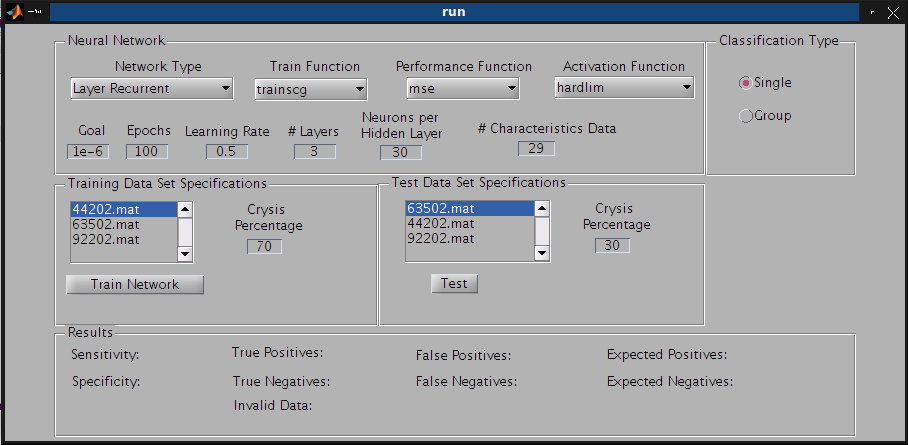
\includegraphics[scale=0.3]{Images/Aplication_GUI.png}
  \caption{Interface Gráfica implementada}
\end{figure}

\subsection{Redes Neuronais Implementadas}

Como já referimos anteriormente, na nossa aplicação implementámos cinco redes neuronais distintas: \emph{Radial Basis Function}, \emph{Layer Recurrent Network}, \emph{FeedForward}, \emph{FeedForward Time Input Delay} e \emph{Distributed Time Delay}.

Estas redes apresentam, naturalmente, características e propriedades distintas, sendo que umas se adequam mais ao trabalho que pretendemos realizar do que outras.

Por exemplo, considerando a rede \emph{Layer Recurrent}, esta rede permite a introdução de atrasos em algumas características, o que lhe permite aprender a prever qualquer saída dinâmica, tendo por base entradas passadas. Este processo é possível se forem considerados neurónios e atrasos suficientes na rede.

De facto, esta é uma propriedade que vai, de certa forma, ao encontro do funcionamento de um cérebro humano, que para além de ser um sistema dinâmico, possui também memória.

Na mesma linha de raciocínio, redes que suportam a introdução de atrasos em algumas das características que constituem os dados de entrada surgem, a uma primeira vista, como boas opções para simular o comportamento de um cérebro humano, realizando uma melhor identificação das situações correspondentes a crises epiléticas. Exemplos destas redes são a rede \emph{Distributed Time Delay} e a \emph{FeedForward Input Time Delay}.

Por seu turno, a rede \emph{FeedForward} também se apresenta como uma solução a considerar, dado o facto de permitir uma boa implementação de qualquer função de entradas e saídas arbitrárias, desde que considerados neurónios suficientes na(s) camada(s) escondida(s).

Por fim, é também necessário referir a rede \emph{Radial Basis Function}, bastante utilizada para aproximar funções e cujo treino passa nomeadamente pela adição de neurónios à camada escondida até que a rede atinja a performance (\emph{goal}) pretendida. Assim, embora possa ser necessário adicionar um elevado número de neurónios à camada escondida, acreditamos ser possível ter uma boa performance com esta rede.

\subsection{Treino das Redes}

Um dos principais aspetos do trabalho realizado, prende-se com o treino das redes neuronais, pois é ele que determina a boa (ou má) performance das redes implementadas.

Para o presente trabalho foram-nos fornecidos dados relativos a três pacientes, constituídos por um conjunto de características extraídas para cada elemento, e pela respetiva classe definida para cada elemento.

Uma vez que as situações em que os pacientes estão a sofrer de uma crise epilética são consideravelmente menos do que as situações em que o paciente não apresenta nenhum problema, a simples seleção de todos os elementos de um dos conjuntos fornecidos, ou de parte desses elementos, para realizar o treino da rede, sem qualquer cuidado na seleção dos elementos irá conduzir a dados de treino onde predominam situações \emph{não-ictais}.

Nesses casos, iremos verificar uma especialização da rede na identificação de situações \emph{não-ictais}, sem que faça uma classificação de casos \emph{ictais} igualmente fiável.

De facto, tal situação não é desejável, uma vez que o nosso principal objetivo passa pela identificação de casos \emph{ictais} com um grau de confiança mínimo, não a identificação de situações \emph{não-ictais}.

Assim, para evitar que as redes por nós treinadas se especializem em situações \emph{não-ictais}, na constituição dos casos de treino das diferentes redes neuronais, consideramos um dos ficheiros fornecidos, e para esse ficheiro selecionamos uma percentagem dos casos \emph{ictais} (essa percentagem é solicitada ao utilizador através da interface gráfica) que vamos incluir no nosso \emph{data set} de treino.

Em seguida, selecionamos um número igual de situações \emph{não-ictais}, preservando a ordem dos diferentes casos nos dados originais: Consideremos os elementos \emph{A} e \emph{B}, pertencentes ao \emph{data set} original e de treino, em que \emph{A} surge antes de \emph{B} no \emph{data set} original. Consideremos também que \emph{A} corresponde a uma situação \emph{ictal}, enquanto \emph{B} corresponde a uma situação \emph{não-ictal}. Então, no \emph{data set} de treino, \emph{A} surgirá também antes de \emph{B}.

Para realizar o treino das diversas redes recorremos ainda a várias 

%Explicar que em todas as redes utilizámos a função train do matlab excepto na newrb, em que o treino é realizado automaticamente pelo matlab aquando da criação da rede.

%Por fim, dizer que o treino foi realizado com recurso à função train da Neural Network Toolbox do Matlab

\subsection{Teste das Redes}

Falar da divisão das crises nos casos de teste: Como ja temos a rede treinada, não temos de ter a preocupação de ter proporções de situações ictais e não-ictais identicas.


\subsection{Implementação em Matlab}

Falar na estrutura dos ficheiros e no ficheiro que é para correr

Falar sobre os ficheiros mais importantes

%createNetwork

%prepareDataSets

%interpretResults e interpretGroupResults

%run

\subsection{Execução}

%Explicar como executar o código

\pagebreak

\section{Treino e Testes da Aplicação}



\pagebreak

\section{Conclusões}


\pagebreak

\section{Anexos}



\end{document}